\documentclass[11pt,a4paper]{article}
\usepackage{amsmath,tikz, amssymb,amsthm, multirow, pgfplots, booktabs, bbm}
\pgfplotsset{compat=1.18}
\usepgfplotslibrary{groupplots}
\usetikzlibrary{decorations.pathreplacing, shapes.arrows, positioning}

\begin{document}

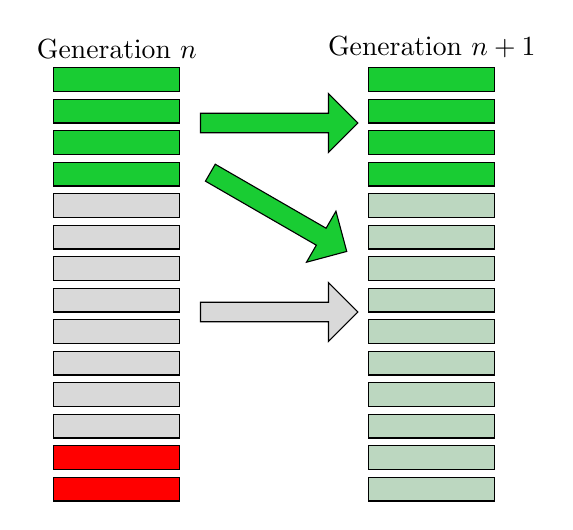
\begin{tikzpicture}[scale=0.4]
	\definecolor{mygreen}{rgb}{0.1,0.8,0.2}
	\definecolor{mygray}{gray}{0.85}

	\foreach \h in {0,...,3}{\draw[fill=mygreen] (0,-\h) rectangle (4,-\h-0.75);}
	\foreach \h in {4,...,11}{\draw[fill=mygray] (0,-\h) rectangle (4,-\h-0.75);}
	\foreach \h in {12,...,13}{\draw[fill=red] (0,-\h) rectangle (4,-\h-0.75);}

	\node[single arrow, draw, fill=mygreen, minimum height=2cm] at (7,-1.75) {};
	\node[single arrow, draw, fill=mygreen, minimum height=2cm, rotate=-30] at (7,-4.5) {};
	\node[single arrow, draw, fill=mygray, minimum height=2cm] at (7,-7.75) {};

	\foreach \h in {0,...,3}{\draw[fill=mygreen] (10,-\h) rectangle (14,-\h-0.75);}
	\foreach \h in {4,...,13}{\draw[fill=mygray!85!mygreen] (10,-\h) rectangle (14,-\h-0.75);}

	\node[above] at (2,0) {Generation $n$};
	\node[above] at (12,0) {Generation $n+1$};
\end{tikzpicture}

\end{document}